\chapter{Interfaz con el portón}
\label{cap:interfaz}

El desarrollo del módulo de control físico requiere definir previamente qué tipo de señales pueden considerarse disponibles en un automatismo residencial representativo. Para ello se analizaron distintas centrales utilizadas en portones corredizos, principalmente de las marcas PPA y SEG, buscando identificar características comunes en la forma de accionar el portón, detectar sus posiciones extremas y alimentar dispositivos auxiliares.

El objetivo de este análisis no es seleccionar una única central como requisito del proyecto, sino establecer una base suficientemente representativa a partir de controladores de uso común. De esta manera, el desarrollo posterior de la interfaz electrónica podrá realizarse sobre señales y modos de operación que aparecen de forma recurrente en distintos equipos, evitando depender desde el inicio de una implementación particular.

\section{Controladores considerados}

Entre las centrales analizadas se encuentra la PPA Triflex Facility, utilizada en distintas líneas de automatizadores de la marca. Su documentación contempla entradas destinadas a finales de carrera y a botoneras externas, además de una alimentación auxiliar disponible para accesorios. Para el final de carrera, la central interpreta el accionamiento cuando la entrada correspondiente es llevada a GND, mientras que la orden proveniente de una botonera se implementa mediante el cierre de contactos sobre las entradas de mando correspondientes.

También se consideraron controladores correspondientes a la familia PPA Pop Connect. Estos equipos mantienen una arquitectura similar desde el punto de vista funcional, al disponer de entradas para el accionamiento externo y de señales destinadas a determinar la posición del portón. La implementación interna y los niveles eléctricos pueden variar respecto de otras centrales, por lo que su consideración resulta útil para no asociar el posterior diseño a un único valor de tensión o a una única disposición de conectores.

Dentro de los automatismos SEG se analizaron principalmente las centrales Wave y G-II. La central Wave dispone de entradas de botonera referenciadas al GND del controlador y de una salida auxiliar de 12~Vcc, limitada a una corriente especificada por el fabricante. Esto permite observar que, además de las señales de mando, existen controladores que proporcionan alimentación destinada a dispositivos externos dentro del mismo dominio eléctrico de la placa.

La central SEG G-II presenta una estructura comparable, con entradas destinadas al accionamiento mediante botonera y una salida auxiliar de 12~Vcc. En este caso la documentación especifica una capacidad de corriente superior y señala que dicha salida no se encuentra regulada, mostrando que la disponibilidad de alimentación auxiliar no implica necesariamente características eléctricas idénticas entre diferentes controladores.

También se tomó como referencia la línea SEG Solo CH, donde el posicionamiento del portón se resuelve mediante sensores magnéticos asociados a los extremos del recorrido. La documentación de esta familia describe el uso de sensores reed normalmente abiertos para la detección de los finales de carrera, confirmando la presencia de una lógica basada en el cambio de estado de un contacto asociado a una entrada de la central.

El análisis conjunto de estos controladores permite identificar una estructura funcional común, aun cuando existan diferencias en tensión, capacidad de corriente, tipo de sensor y disposición física de los terminales.

\section{Señales disponibles en las centrales}

\subsection{Final de carrera}

Para SmartGate resulta necesario conocer si el portón se encuentra completamente cerrado antes de generar una nueva orden de apertura. En lugar de incorporar un sensor de posición independiente, se toma como base el aprovechamiento del sistema de final de carrera ya presente en el automatismo.

En las centrales analizadas, la posición extrema se determina a partir del cambio de estado de una entrada asociada al sensor de final de carrera. En diferentes implementaciones este sensor puede encontrarse constituido por un contacto mecánico, un relé o un sensor magnético reed, pero funcionalmente la central recibe una modificación de nivel eléctrico cuando el portón alcanza la posición correspondiente.

Como representación general, se considerará una entrada de referencia asociada al final de carrera y referenciada al GND de la central. Entre dicha entrada y GND se encuentra el contacto seco del sensor. Cuando este contacto permanece abierto, sobre la entrada puede existir una tensión de control determinada por la electrónica interna del controlador, o bien presentarse un estado de alta impedancia. Al accionarse el final de carrera, el contacto cierra el circuito y establece la conexión de dicha entrada hacia GND.

De forma conceptual:

\begin{center}
\texttt{REF\_FC} $\rightarrow$ contacto de final de carrera $\rightarrow$ \texttt{GND}
\end{center}

El valor de tensión presente en \texttt{REF\_FC} con el contacto abierto no se considerará único, dado que depende de la electrónica interna de cada controlador. En los equipos analizados aparecen diferentes niveles de alimentación y arquitecturas, por lo que esta entrada podrá encontrarse polarizada a un determinado nivel de control o permanecer en alta impedancia. En consecuencia, esta señal se tratará posteriormente como una variable de interfaz y no como un nivel lógico fijo.

Para el proyecto únicamente interesa recuperar la información correspondiente al final de carrera de cierre. De esta manera, SmartGate podrá conocer el estado físico del portón utilizando el mismo elemento que emplea la central original para determinar que el recorrido de cierre ha finalizado.

\subsection{Accionamiento del portón}

La segunda señal de interés corresponde al comando utilizado para solicitar un movimiento del portón. Los controladores considerados disponen de entradas destinadas a botoneras, pulsadores o dispositivos externos, permitiendo actuar sobre el automatismo sin intervenir directamente en su etapa de potencia.

En términos funcionales, estas entradas operan mediante el cierre temporal de un contacto entre la entrada de mando y la referencia de GND de la central. Este comportamiento es equivalente al producido por una botonera convencional instalada en paralelo con otros medios de accionamiento.

Como representación general se considerará:

\begin{center}
\texttt{BTN} $\rightarrow$ contacto temporal $\rightarrow$ \texttt{GND}
\end{center}

La utilización de esta entrada resulta especialmente conveniente para SmartGate porque permite que el sistema externo únicamente genere una solicitud de accionamiento. La interpretación de dicha solicitud, la secuencia de movimiento del motor, la actuación de los finales de carrera y las demás funciones propias del automatismo continúan siendo gestionadas por la central original.

De esta forma, la integración se realiza sobre una interfaz que ya ha sido prevista por el fabricante para mandos externos, sin necesidad de actuar directamente sobre relés de potencia, bobinados del motor u otros elementos internos del controlador.

\subsection{Alimentación auxiliar}

Otro aspecto observado durante el análisis es la disponibilidad de salidas auxiliares de alimentación en distintas centrales. Estas salidas se utilizan habitualmente para alimentar fotocélulas, receptores, sensores u otros accesorios asociados al automatismo.

En la central PPA Triflex Facility se dispone de una salida auxiliar de 15~Vcc, mientras que en las centrales SEG Wave y SEG G-II aparecen salidas de 12~Vcc con diferentes capacidades de corriente. Esto muestra que es frecuente disponer dentro de la propia central de una fuente de continua referenciada a su GND, aunque sus características concretas dependen del modelo utilizado.

La existencia de este tipo de alimentación resulta relevante para el desarrollo posterior, ya que permite considerar la posibilidad de alimentar la electrónica asociada al lado del portón desde el propio dominio eléctrico de la central. Sin embargo, la tensión disponible, su regulación y la corriente máxima deberán considerarse individualmente para cada controlador.

\section{Base adoptada para el diseño}

A partir de las centrales estudiadas se tomará como base una arquitectura en la que el portón dispone de una referencia eléctrica común asociada a su controlador, una señal de final de carrera de cierre y una entrada destinada al accionamiento mediante botonera.

La detección de portón cerrado se realizará a partir del cambio de estado de la señal utilizada por el propio final de carrera, mientras que la orden de movimiento se generará reproduciendo eléctricamente el comportamiento de un pulsador externo entre la entrada de mando y GND.

Asimismo, se considerará posible la existencia de una alimentación auxiliar dentro del dominio eléctrico de la central, con valores que pueden encontrarse aproximadamente en el entorno de 12 a 15~Vcc según el controlador utilizado.

Estas condiciones establecen la base funcional y eléctrica sobre la cual se desarrolla la interfaz de SmartGate, cuyo circuito de lectura del final de carrera y su implementación en placa se describen a continuación.

\section{Interfaz de lectura del final de carrera}

La lectura del estado del final de carrera se plantea mediante una interfaz conectada en paralelo con la señal original del portón, procurando que su incorporación no modifique el funcionamiento normal del controlador. El circuito actúa de esta forma como un \textit{sniffer} de la señal asociada al contacto magnético, limitando la corriente intercambiada con la entrada original y manteniendo aislada eléctricamente la Raspberry Pi respecto de la electrónica del automatismo.

Para el diseño se consideran dos posibles comportamientos de la entrada de final de carrera cuando el contacto se encuentra abierto. En el primer caso, la controladora puede incorporar internamente una resistencia de pull-up, manteniendo el pin a una tensión lógica propia. En el segundo, la entrada puede permanecer en un estado de alta impedancia, dependiendo exclusivamente del cierre del contacto hacia masa para detectar el final de carrera. En ambos casos, al accionarse el sensor, la señal se establece próxima a GND.

Con el objetivo de contemplar ambas posibilidades sin imponer directamente la tensión de alimentación sobre una entrada cuya electrónica interna es desconocida, se incorpora una polarización débil hacia aproximadamente 3,3~V. Esta tensión se obtiene a partir de la menor alimentación prevista para la controladora, $V_{CC} = 12$~V, mediante un divisor resistivo de elevada impedancia. Si la tensión disponible en el automatismo fuera superior, deberá acondicionarse previamente para conservar este mismo nivel de polarización.

La elevada resistencia equivalente del divisor hace que, cuando la controladora posee un pull-up propio, sea principalmente la electrónica original la que determine la tensión del nodo. Por ejemplo, frente a resistencias internas del orden de 10~k$\Omega$ a 47~k$\Omega$, una red externa con una resistencia equivalente cercana a 100~k$\Omega$ introduce únicamente una carga reducida y no modifica de forma significativa el nivel lógico establecido por la placa. En cambio, si la entrada se encuentra en alta impedancia, esta misma red fija el nodo en torno a 3,3~V, evitando que la entrada del comparador quede flotante. De esta forma se obtiene un comportamiento definido para ambas arquitecturas sin aplicar directamente 12~V sobre el pin de final de carrera.

La señal obtenida se compara con una referencia de aproximadamente 1,3~V. Mientras el contacto permanece abierto, la entrada se mantiene por encima de este umbral, ya sea debido a la polarización interna de la controladora o a la red auxiliar de 3,3~V. Cuando el final de carrera conecta la señal a masa, la tensión desciende por debajo de la referencia y el comparador conmuta. Para esta función se prevé utilizar un LM393, cuya salida de colector abierto permite controlar directamente la corriente del LED de un optoacoplador.

La salida del comparador gobierna un PC817 mediante una resistencia serie de 1,5~k$\Omega$. El transistor de salida del optoacoplador pertenece a un circuito eléctricamente independiente, alimentado a 3,3~V desde el lado de la Raspberry Pi. En este sector se utiliza una resistencia de pull-up de 3,3~k$\Omega$, de forma que el estado de conducción del PC817 se transforma en un nivel lógico adecuado para una entrada GPIO.

Esta separación mediante optoacoplador evita compartir la referencia de masa entre el controlador del portón y la Raspberry Pi. De esta forma, cualquier diferencia de potencial, ruido o perturbación presente en la electrónica de potencia queda desacoplada del sistema de procesamiento. En conjunto, la elevada impedancia de la etapa de sensado y el aislamiento óptico permiten obtener información del final de carrera con una influencia mínima sobre el circuito original y sin establecer una conexión eléctrica directa con la Raspberry Pi.

\section{Implementación de la placa de interfaz}

A partir del análisis de las señales disponibles se diseñó y fabricó una placa de circuito impreso (PCB) por parte del equipo en las instalaciones de la Universidad ORT Uruguay. La placa concentra en una única solución las conexiones necesarias para vincular la Raspberry Pi con la central del portón, los finales de carrera, los indicadores y los actuadores. El uso de borneras facilita el montaje y el mantenimiento, mientras que los zócalos permiten reemplazar componentes sin intervenir directamente sobre las pistas.

Esta implementación permitió pasar del esquema conceptual a un módulo físico reproducible y ordenado. Además de reducir conexiones sueltas durante las pruebas, la PCB establece puntos de entrada y salida definidos, simplifica el diagnóstico y deja una base adecuada para futuras revisiones del hardware.

\begin{figure}[H]
    \centering
    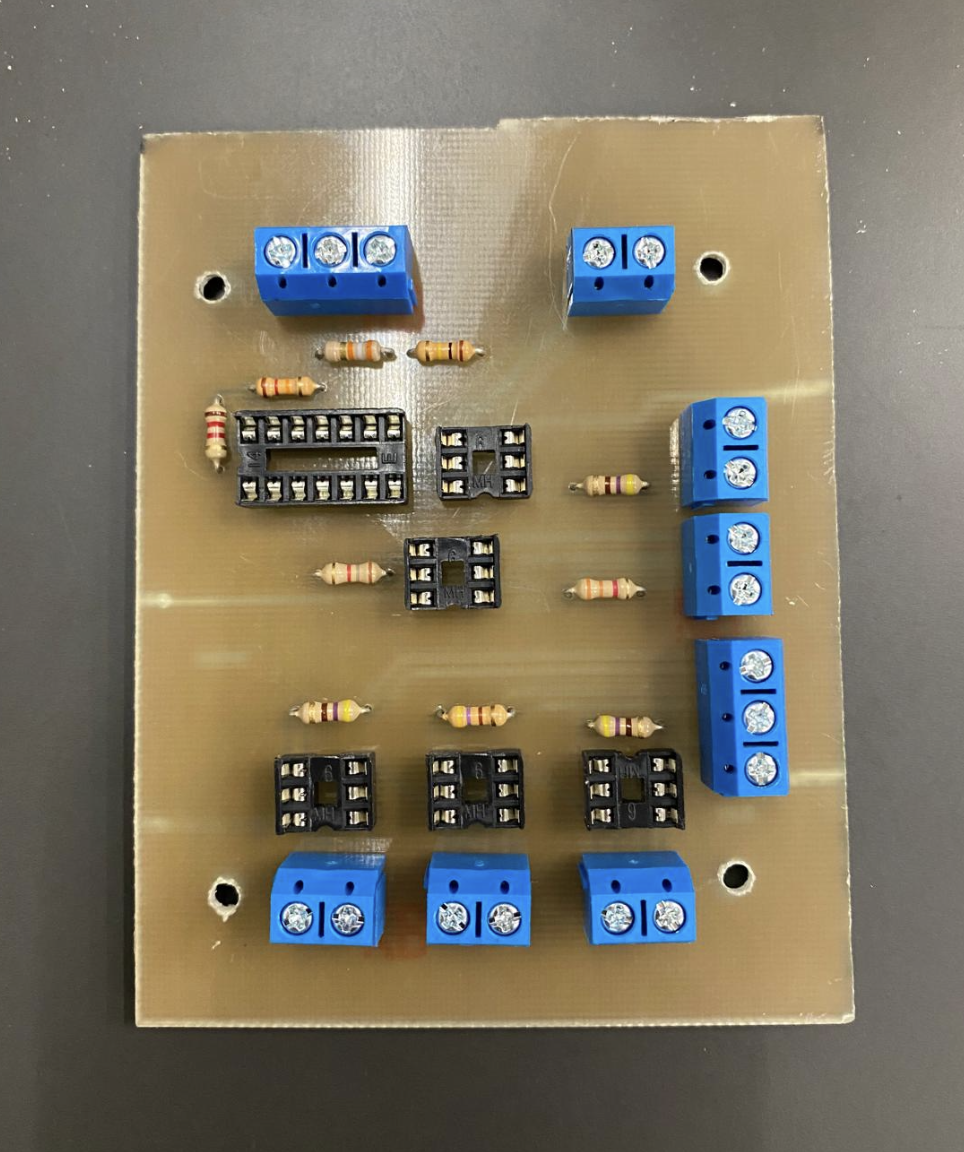
\includegraphics[width=0.6\textwidth]{Imagenes/pcb_interfaz.png}
    \caption{PCB de interfaz desarrollada y fabricada por el equipo en la Universidad ORT Uruguay.}
    \label{fig:pcb}
\end{figure}
